\documentclass{beamer}

\setbeamertemplate{footline}[frame number]
\setbeamertemplate{navigation symbols}{}
\usetheme{Madrid}
\begin{document}

\title{Dataset and Data Register download tools}
\author{zhang gang}
\institute{IHEP}

\maketitle

\begin{frame}
      \frametitle{Outline}
      \tableofcontents
\end{frame}

\section{Dataset problems}
\begin{frame}
  \frametitle{New dataset methods}
  \begin{itemize}
    \item New dataset methods show
  \end{itemize}
  \hspace{0.5cm} 
  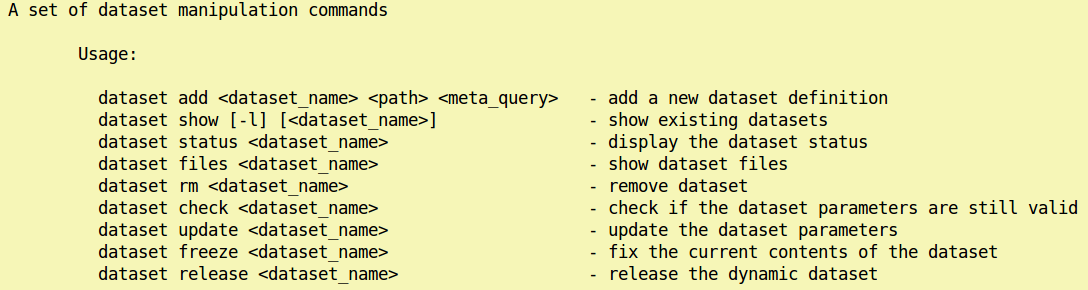
\includegraphics[height=4cm,width=11cm,keepaspectratio]{data/datasetMethod.png}
  \begin{itemize}
    \item Two new tables: FC\_MetaDatasets and FC\_MetaDatasetFiles
    \item I have test these dataset methods. All of them is useable,but I meet some problem for our use 
  \end{itemize}
\end{frame}

\begin{frame}
  \frametitle{Describe tables}
  \begin{itemize}
    \item Abundant fields to describe a dataset 
  \end{itemize}
  \hspace{0.5cm} 
  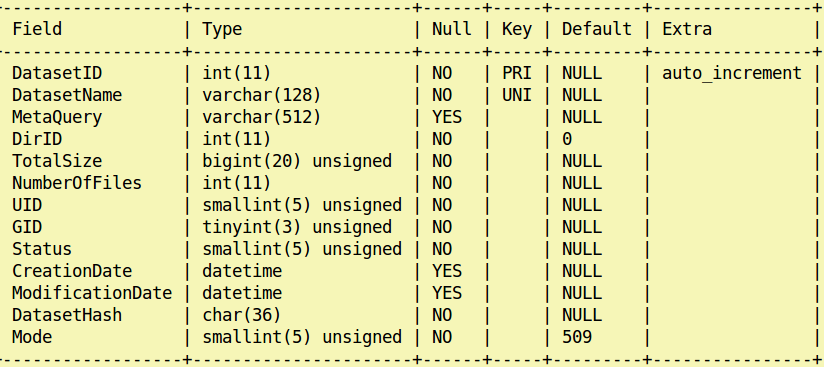
\includegraphics[height=4cm,width=11cm,keepaspectratio]{data/FC_MetaDatasets.png}
  \begin{itemize}
    \item We can get some useful information from these fields,like UID,GID... 
    \item Maybe we coule use these fields to intensify our tools,like let user create their own datasets
    \item Discuss: Naming rule of dataset,who have the right to create dataset...
  \end{itemize}
\end{frame}

\begin{frame}
  \frametitle{Matadata Manager}
  \begin{itemize}
    \item Problem:Add file level metadata in metaquery when create a datasetname, match 0 files
    \item List the all metadatas and find the problem:field 'runL' 'runH' are both fileMetaField and directoryMetaFields which
      result in the unmatch problem
  \hspace{0.5cm} 
  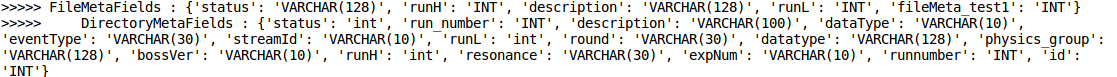
\includegraphics[height=10cm,width=15cm,keepaspectratio]{data/metaShow.png}
  %k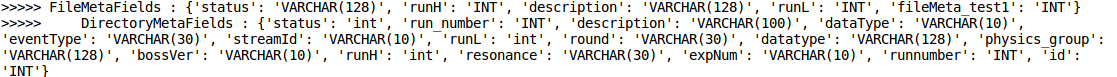
\includegraphics[keepaspectratio]{data/metaShow.png}
    \item Discuss: How to manager metadata
      \begin{itemize}
        \item Naming rule: Avoid two fields have the same meaning
        \item Manager: Only authorized persion can change meta fields
      \end{itemize}
  \end{itemize}
\end{frame}
\section{Data upload and download tools}
\begin{frame}
  \frametitle{The location of files}
  \begin{itemize}
    \item Upload data
      \begin{itemize}
          \item LFN:/bes/File/jpsi/6.6.4/data/all/round02   15581 files   about 7.7TB
          \item LFN:/bes/File/jpsi/6.6.4/mc/inclusive/round02 4709 files  about 3.7TB
          \item Relevant metadatas: User can create dataset with them
            \begin{itemize}
              \item Directorymetafields: resonance,bossVer,eventType,round
              \item Filemetafields:runL,runH
            \end{itemize}
      \end{itemize}
    \item Download data: total about 1.5TB
      \begin{itemize}
          \item AFS:../psipp/664p01/mc/DpDm/round03/stream001/
          \item AFS:../psipp/664p01/mc/nonqq/round03/stream001/
          \item AFS:../psipp/664p01/mc/gammaJpsi/round03/stream001/
          \item AFS:../psipp/664p01/mc/gammapsip/round03/stream001/
          \item AFS:../psipp/664p01/mc/ditau/round03/stream001/
          \item AFS:../psipp/664p01/mc/qqbar/round03/stream001/
      \end{itemize}
  \end{itemize}
\end{frame}

\begin{frame}
  \frametitle{How to download files for user}
  \begin{itemize}
    \item Provide three ways to download data 
      \begin{itemize}
          \item By dataset name
            \begin{itemize}
                \item User can download a whole dataset
                \item Example: besdirac-upload-files datasetName
            \end{itemize}
          \item By meta query 
            \begin{itemize}
                \item Download data by a dynamic query condition
                \item Example: besdirac-upload-files resonance=jpsi bossVer=6.6.3 runL$>$100 runH$<$200 runL!=150
            \end{itemize}
          \item By dir in DFC
            \begin{itemize}
                \item Download files under a given DFC dir
                \item Example: besdirac-upload-files /bes/File/4260/6.6.3/data/all/round06 
            \end{itemize}
      \end{itemize}
  \end{itemize}
\end{frame}

\begin{frame}
  \frametitle{Optimize tools}
  \begin{itemize}
    \item Handle failed files 
      \begin{itemize}
          \item Add a global error list, if file transfer failed, add the file to the list
          \item After the transfer, check error list, if not null, the retransfer files in list 
      \end{itemize}
    \item File checksum 
      \begin{itemize}
          \item First check the adler32 value of each file on SE and local dir, slow
          \item Change to check the size of each of file, very fast
          \item if not equal,then retransfer the file
      \end{itemize}
  \end{itemize}
\end{frame}
\end{document}
